\documentclass[border=10pt]{standalone}

\usepackage{tikz}
\usepackage{tikzsymbols}
\usetikzlibrary{calc,patterns,shapes.geometric}

\def\centerarc[#1](#2)(#3:#4:#5){\draw[#1] ($(#2)+({#5*cos(#3)},{#5*sin(#3)})$) arc (#3:#4:#5);}

\begin{document}
	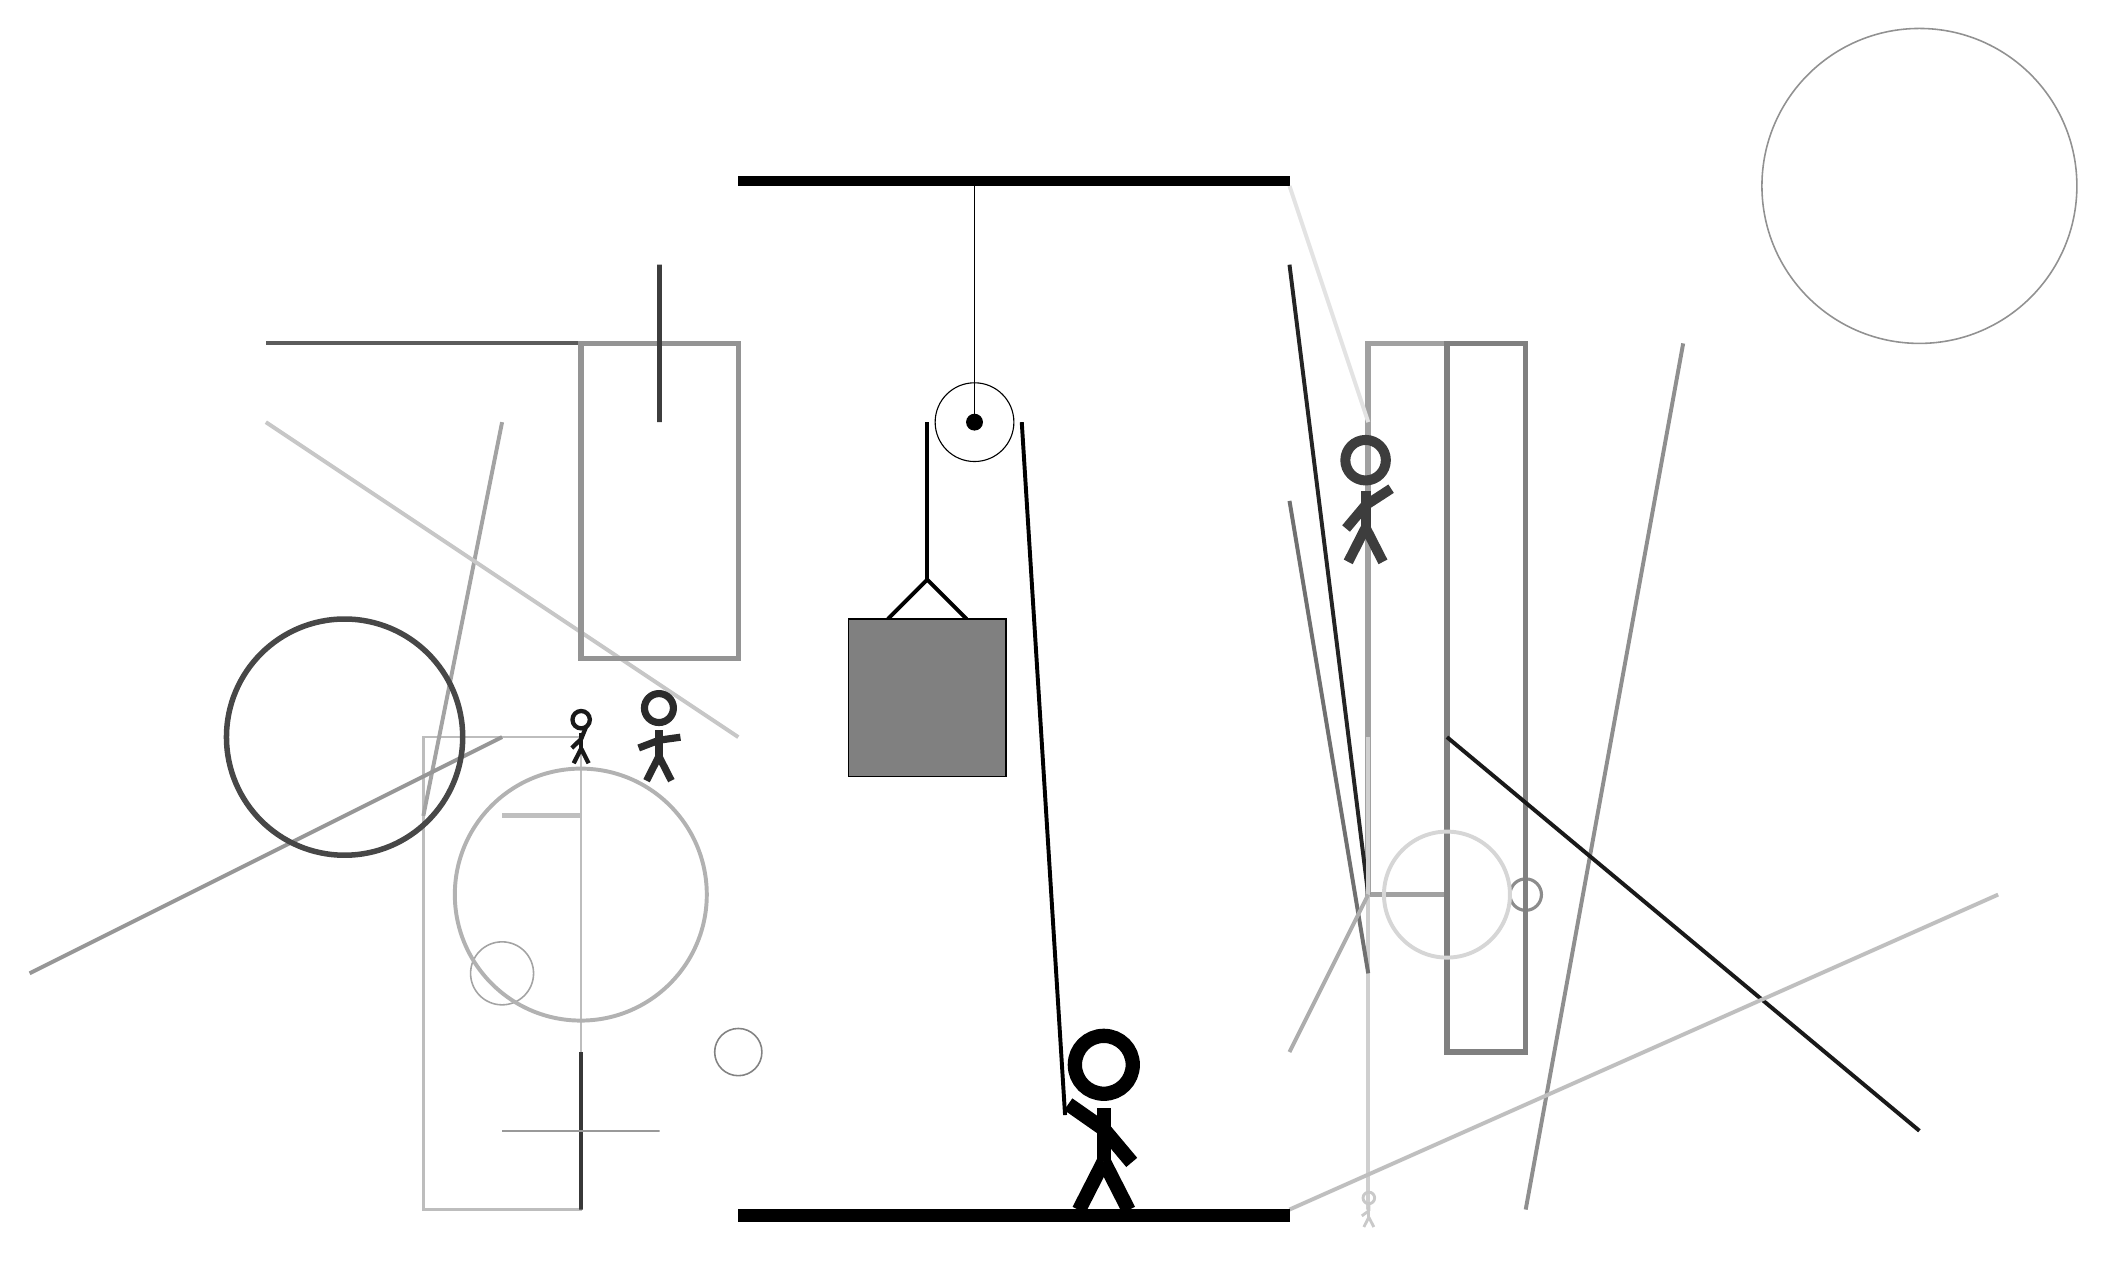
\begin{tikzpicture}
		%%%%% START %%%%%
		
		\draw[fill=black] (-2, 10) rectangle (5, 10.125);
		
		\draw (1, 7) circle (0.5);
		\draw[fill=black] (1, 7) circle (0.1);
		\draw (1, 10) -- (1, 7);
		
		\draw[line width=0.5mm] (-0.1, 4.5) -- (0.4, 5.0) -- (0.9, 4.5);
		\draw[fill=black!50] (-0.6, 4.5) rectangle (1.4, 2.5);
		
		\draw[line width=0.5mm] (0.4, 7) -- (0.4, 5.0);
		\centerarc[line width=0.5mm](1, 7)(0:180:0.6);
		\draw[line width=0.5mm](1.6, 7) -- (2.15, -1.8);
		
		\draw[line width=0.7mm, color=black!37] (7, 1) rectangle (6, 8);
		
		\draw[line width=0.6mm, color=black!25] (-4, 2) rectangle (-5, 2);
		\node[line width=0.4mm, color=black!76] at (6, 6) {\Strichmaxerl[7][50][33]};
		\draw[line width=0.5mm, color=black!86](5, 9) -- (6, 1);
		\draw [line width=0.2mm, color=black!49](-2, -1) circle (0.3);
		
		\draw[line width=0.3mm, color=black!26] (-4, 3) rectangle (-6, -3);
		\draw[line width=0.5mm, color=black!19] (6, 3) rectangle (6, -3);
		\draw[line width=0.5mm, color=black!36](-6, 2) -- (-5, 7);
		\draw[line width=0.5mm, color=black!44](10, 8) -- (8, -3);
		\draw [line width=0.2mm, color=black!36](-5, 0) circle (0.4);
		
		\node[line width=0.5mm, color=black!21] at (6, -3) {\Strichmaxerl[2][36][88]};
		\draw[line width=0.5mm, color=black!22](-2, 3) -- (-8, 7);
		\draw [line width=0.4mm, color=black!45](8, 1) circle (0.2);
		\draw[line width=0.7mm, color=black!50] (7, -1) rectangle (8, 8);
		\draw [line width=0.5mm, color=black!16](7, 1) circle (0.8);
		\draw[line width=0.5mm, color=black!41](-5, 3) -- (-11, 0);
		\draw[line width=0.5mm, color=black!56](6, 0) -- (5, 6);
		\draw[line width=0.5mm, color=black!64](-3, 8) -- (-8, 8);
		\draw[line width=0.7mm, color=black!42] (-4, 4) rectangle (-2, 8);
		\draw[line width=0.5mm, color=black!78] (-4, -3) rectangle (-4, -1);
		\draw[line width=0.6mm, color=black!76] (-3, 9) rectangle (-3, 7);
		
		\node[line width=0.4mm, color=black!90] at (-4, 3) {\Strichmaxerl[3][44][68]};
		\draw [line width=0.5mm, color=black!30](-4, 1) circle (1.6);
		\draw[line width=0.5mm, color=black!90](7, 3) -- (13, -2);
		\draw[line width=0.5mm, color=black!25](5, -3) -- (14, 1);
		
		\node[line width=0.5mm, color=black!83] at (-3, 3) {\Strichmaxerl[5][21][8]};
		
		\draw[line width=0.3mm, color=black!40] (-3, -2) rectangle (-5, -2);
		\draw [line width=0.2mm, color=black!43](13, 10) circle (2.0);
		\draw[line width=0.5mm, color=black!11](5, 10) -- (6, 7);
		\draw[line width=0.5mm, color=black!32](5, -1) -- (6, 1);
		\draw [line width=0.7mm, color=black!72](-7, 3) circle (1.5);
		
		
		\node at (2.6, -1.9) {\Strichmaxerl[10][-35][-50]};
		
		\draw[fill=black] (-2, -3) rectangle (5, -3.15);
		
		%%%%% END %%%%%
	\end{tikzpicture}
\end{document}